% Beamer do material do curso de Verão (2015) do IME-USP
% Introdução ao Projeto de Jogos
%
% Baseado no template LaTeX das apresentações do LIDET versão 2
% (https://github.com/luigivieira/LIDET)
%

\providecommand\classopts{}
\expandafter\documentclass\expandafter[table, usenames, svgnames, dvipsnames, \classopts]{beamer}

\usepackage{etex}
\usepackage{beamerthemeshadow}
\usepackage[portuguese]{babel}
\usepackage[utf8]{inputenc}
\usepackage[absolute,overlay]{textpos}
\usepackage{array}
\usepackage{framed}
\usepackage{booktabs}
\usepackage{caption}
\usepackage{subcaption}
\usepackage{outlines}
\usepackage{ulem}
\usepackage{xcolor,colortbl}
\usepackage{ragged2e}
\usepackage{tikz}

\captionsetup{compatibility=false}

% ---------------------------------------------------------------------------- %
% Presentation definitions
% ---------------------------------------------------------------------------- %
\usetheme{Luebeck}
\hypersetup{pdfpagemode=FullScreen} % Starts the presentation in full screen

% layout
\setbeamerfont{frametitle}{size=\normalsize}
\setbeamerfont{title}{size=\normalsize}
\beamertemplatenavigationsymbolsempty
\setbeamertemplate{bibliography item}[text]%

% colors
\definecolor{lidet_orange}{rgb}{0.9, 0.49, 0.09}
\definecolor{lidet_black}{rgb}{0.2, 0.2, 0.2}

\setbeamercolor{title}{bg=lidet_orange}
\setbeamercolor{structure}{bg=white, fg=lidet_orange}
\setbeamercolor{normal text}{fg=black}
\setbeamercolor{section in head/foot}{fg=white, bg=lidet_black}
\setbeamercolor{postit}{fg=white, bg=lidet_orange!90!lidet_black}

% shadow
\makeatletter
\pgfdeclareverticalshading[black,bg]{bmb@shadow}{200cm}{%
  color(0bp)=(lidet_black!25); color(4bp)=(black!50!bg); color(8bp)=(black!50!bg)}
\pgfdeclareradialshading[black,bg]{bmb@shadowball}{\pgfpointorigin}{%
  color(0bp)=(black!50!bg); color(4bp)=(lidet_black!25)}
\pgfdeclareradialshading[black,bg]{bmb@shadowballlarge}{\pgfpointorigin}{%
  color(0bp)=(black!50!bg); color(4bp)=(black!50!bg); color(8bp)=(lidet_black!25)}
%
\makeatother

% Captions for images and tables
\setlength{\abovecaptionskip}{5pt plus 5pt minus 5pt}
\setlength{\belowcaptionskip}{5pt plus 5pt minus 5pt}
\captionsetup[figure]{font=scriptsize,labelfont=scriptsize}
\captionsetup[table]{font=scriptsize,labelfont=scriptsize}
\captionsetup{labelformat=empty,labelsep=none}

% Dimensions for table rules
\setlength\heavyrulewidth{0.1em} 
\setlength\lightrulewidth{0.01em}
\setlength\belowrulesep{0.10ex}
\setlength\aboverulesep{0.10ex}

% Define macros to mark the begining and ending of references
% Basically, handles the automatically spanned frames (due to parameter allowframebreaks)
% as backup frames, so they do not influence in the frame numbering
\newcommand{\referencesbegin}{
   \newcounter{framenumberappendix}
   \setcounter{framenumberappendix}{\value{framenumber}}
}
\newcommand{\referencesend}{
   \addtocounter{framenumberappendix}{-\value{framenumber}}
   \addtocounter{framenumber}{\value{framenumberappendix}} 
}

% Section frames (that appear before each section)
\AtBeginSection[] 
{
	{
		\setbeamertemplate{footline}{} % Hide the footline locally for these frames
		\begin{frame}<beamer>[noframenumbering]
			\begin{center}
				\begin{tikzpicture}
					\node[align=left, left color=lidet_orange, right color=lidet_orange, draw, rounded corners, minimum width=10cm, minimum height=1cm] {\color{white} \textbf{\insertsectionhead}};
				\end{tikzpicture}
			\end{center}
			\footnotesize{ \tableofcontents[currentsection, hideothersubsections] }
		\end{frame}
	}
}

\DeclareGraphicsExtensions{.pdf,.jpg,.png}
\graphicspath{{./images/}}

% ---------------------------------------------------------------------------- %
% Presentation title, author and institution
% ---------------------------------------------------------------------------- %
\title{\textbf{Introdução ao Projeto de Jogos}}
\subtitle{{\small Aula 1 - Enxergando Jogos como Sistemas}}

\author[Luiz Carlos Vieira]{\scriptsize
    Luiz Carlos Vieira e Vinícius Kiwi Daros\\
    \{luigivieira,vinicius.k.daros\}@gmail.com
}

\institute[LIDET (IME - USP)]{\\[1.0mm] 
Curso de Verão (2015)\\
Departamento de Ciência da Computação}

\date{{\tiny 12 de Janeiro de 2015}}

% ---------------------------------------------------------------------------- %
% Presentation content
% ---------------------------------------------------------------------------- %

% ---------------------------------------------------------------------------- %
\begin{document}
% ---------------------------------------------------------------------------- %

% ---------------------------------------------------------------------------- %
% First Slide (index 0) = cover
% ---------------------------------------------------------------------------- %

{%\usebackgroundtemplate{}} 
\begin{frame}[plain, noframenumbering]

	\begin{columns}[c]
		\column{0.2\textwidth}
			\hspace*{-1.5em}
			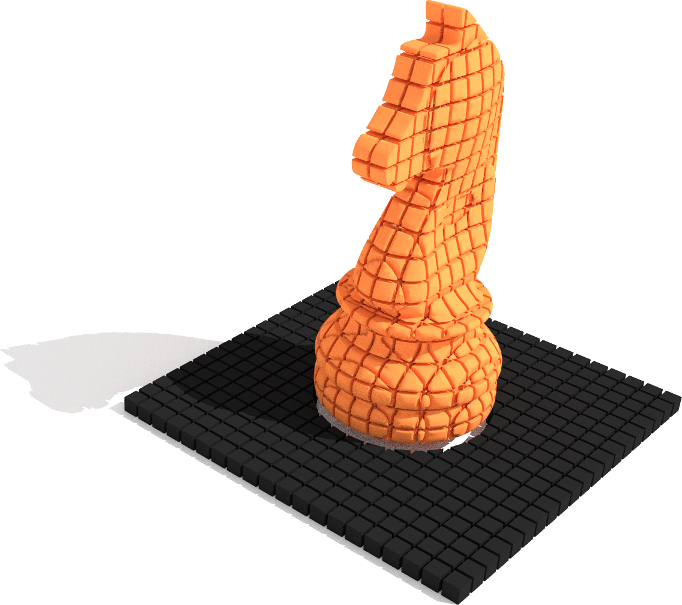
\includegraphics[width=0.35\paperwidth]{side_bar}\\
		\column{0.01\textwidth}
		\column{0.70\textwidth}
			\titlepage
			\hspace*{+0.5em}
			\begin{center}
				
\includegraphics[height=1.0cm]{lidet-logo}\\
				
\includegraphics[height=1.0cm]{ime-logo}\\
			\end{center}
	\end{columns}
	%\addtocounter{framenumber}{-1}
\end{frame}
}

% ---------------------------------------------------------------------------- %
% Other Slides (index from 1 onwards)
% ---------------------------------------------------------------------------- %

% setup navigation symbols and footline
\setbeamertemplate{navigation symbols}{}
\setbeamertemplate{footline}{
   \begin{beamercolorbox}[ht=4ex,leftskip=.3cm,rightskip=.3cm]{author in head/foot}
    %\usebeamercolor{lidet_orange}
    \hrule
    \vspace{0.1cm}
    \insertdate \hfill \insertframenumber/\inserttotalframenumber \newline
    \insertshortauthor \ - \inserttitle \hfill \insertshortinstitute
   \end{beamercolorbox}
   \vspace*{0.1cm}
} 

% ---------------------------------------------------------------------------- %
\begin{frame}[plain]
\frametitle{\textbf{Agenda}}

	\hspace*{+4.0em}
	\footnotesize{ \tableofcontents }
\end{frame}

% ---------------------------------------------------------------------------- %
\section{Sobre o Curso}
% ---------------------------------------------------------------------------- %

\subsection{Provimento}

% ------------------------------
\begin{frame}
	\frametitle{\textbf{Laboratório}}
	
	\begin{center}
		
\includegraphics[height=0.2\paperheight]{lidet-logo}
	\end{center}
	\begin{outline}
		\1 Criado e gerido pelo Prof. Dr. Flávio Soares Corrêa da Silva
			\2[-] {\scriptsize origem no LIAMF (Laboratório de Inteligência Artificial e Métodos Formais)}
			\2[-] {\scriptsize dentro do Departamento de Ciência da Computação do IME-USP}
		
		\1 Pesquisas em interatividade e entretenimento digital
			\2[-] {\scriptsize governo eletrônico, interoperabilidade entre museus, inteligência artificial em jogos eletrônicos, avaliação de experiência de jogadores}
	\end{outline}	

\end{frame}

% ------------------------------
\begin{frame}
	\frametitle{\textbf{Ministrantes}}
	
	\begin{columns}[c]
		\column{0.5\textwidth}
			\begin{center}
				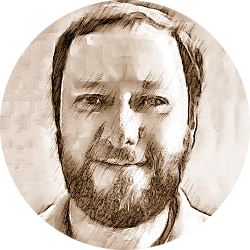
\includegraphics[height=0.3\paperheight]{luiz}\\
				\textbf{Luiz Carlos Vieira}
			\end{center}
			\begin{outline}
				\1 {\scriptsize Doutorando em Ciência da Computação}
					\2[-] {\tiny avaliação de diversão em jogos digitais por meio do rastreamento e análise de expressões faciais}
				
				\1 {\scriptsize Projetista de jogos de tabuleiro}
					\2[-] {\tiny coautor de Turned (publicado na Europa), Xôôô Peste e Reviravolta (em publicação)}
			\end{outline}
		
		\column{0.5\textwidth}
			\begin{center}
				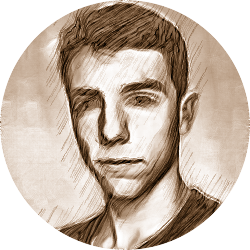
\includegraphics[height=0.3\paperheight]{vinicius}\\
				\textbf{Vinícius Kiwi Daros}
			\end{center}
			\begin{outline}
				\1 {\scriptsize Mestrando em Ciência da Computação}
					\2[-] {\tiny construção de pilotos virtuais com aprendizado de máquina em simuladores automobilísticos}
				
				\1 {\scriptsize Integrante do USP Game Dev}
					\2[-] {\tiny grupo de pesquisa e desenvolvimento de jogos digitais e analógicos}
			\end{outline}
		
	\end{columns}	

\end{frame}

\subsection{Bibliografia Sugerida}

% ------------------------------
\begin{frame} 
	\frametitle{\textbf{Bibliografia sugerida para o curso}}
	
	\begin{columns}[c]
		\column{0.33\textwidth}
			\begin{center}
				\frame{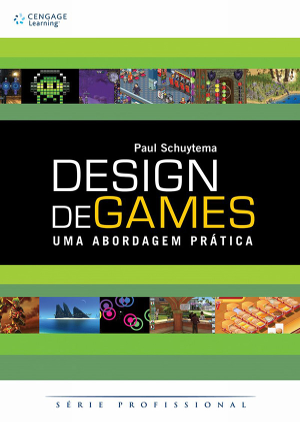
\includegraphics[height=0.5\paperheight]{schuytema}}\\
				Paul Schuytema\\
				\textit{Game Design: Uma Abordagem Prática}\\
				Cengage Learning, 2008
			\end{center}
		\column{0.33\textwidth}
			\begin{center}
				\frame{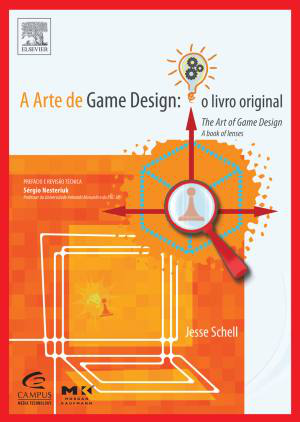
\includegraphics[height=0.5\paperheight]{schell}}\\
				Jesse Schell\\
				\textit{A Arte De Game Design: O Livro Original}\\
				Singular Digital, 2010
			\end{center}
		\column{0.33\textwidth}
			\begin{center}
				\frame{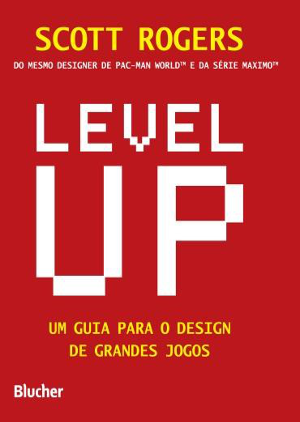
\includegraphics[height=0.5\paperheight]{rogers}}\\
				Scott Rogers\\
				\textit{Level UP: Um Guia para o Design de Grandes Jogos}\\
				Blucher, 2013
			\end{center}
	\end{columns}		
	
\end{frame}



% ------------------------------------------
% References
% ------------------------------------------

%\referencesbegin
%\begin{frame}[plain, allowframebreaks]
%	\frametitle{\textbf{References}}
%	\bibliographystyle{abbrv}
%	{\tiny \bibliography{bibliography}}
%\end{frame}
%\referencesend


% ---------------------------------------------------------------------------- %
% Last Slide = cover + thanks
% ---------------------------------------------------------------------------- %

\institute{
	\begin{center}
		\LARGE{Obrigado!}\\[3.0mm]
	\end{center}
}
\date{}
{%\usebackgroundtemplate{}} 
\begin{frame}[plain, noframenumbering]
	\begin{columns}[c]
		\column{0.2\textwidth}
			\hspace*{-1.5em}
			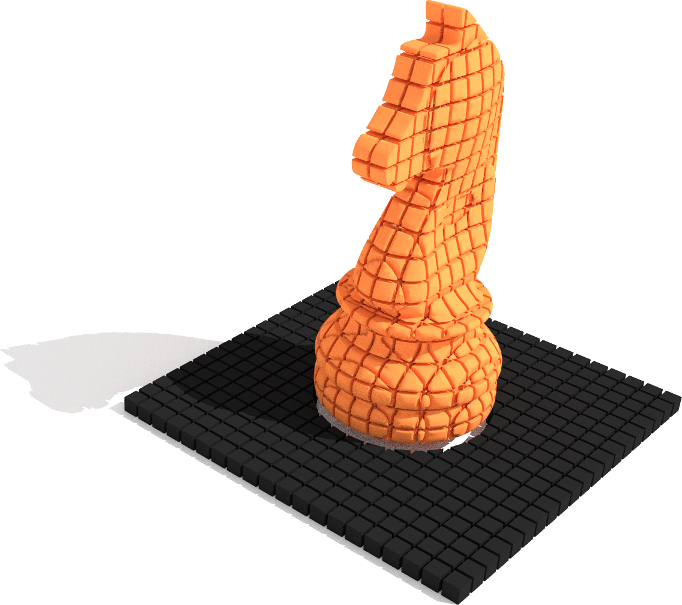
\includegraphics[width=0.35\paperwidth]{side_bar.png}
		\column{0.01\textwidth}
		\column{0.70\textwidth}
			\titlepage
			\begin{center}
				
\includegraphics[height=1.0cm]{lidet-logo}\\
				
\includegraphics[height=1.0cm]{ime-logo}\\				
			\end{center}
	\end{columns}
\end{frame}
}

\end{document}

